\subsection{Arquitectura de IDSs}

Antes de describir los modelos con los que son desarrollados los IDSs, hay que hacer mención de que las técnicas utilizadas por estos sistemas para la detección, no pueden ser generalizadas en un mismo modelo, debido al intento de mejorar un mejor análisis y una mejor clasificación de los datos que este sistema recibe, ha provocado que se puedan implementar diferentes ramas científicas con este enfoque y así intentar la implementación de nuevas técnicas aplicables a los Sistemas de Detección.\\ 

	\subsubsection{Dorothy Denning}
	
	Este modelo de IDS fue propuesto por Dorothy Denning, en donde se explica mediante similitudes informáticas qué es lo que cada componente representa en un IDS. El modelo es enfocado sobre el análisis de un sólo equipo y no de una red. Se constituye por:\\

	\begin{itemize}
		\item Sujetos: Hace referencia a los usuarios de un proceso, sistema o equipo de cómputo.
		\item Objetos: Son los dispositivos periféricos, procesos de sistema, dispositivos de almacenamiento, archivos, aplicaciones de cómputo, entre otros.
		\item Registro de Auditoria: Es el registro obtenido de una interacción de un sujeto sobre los objetos.
		\item Perfiles: Es un comportamiento registrado o patrón de comportamiento que se establecen previamente de la interacción que tiene un sujeto sobre los objetos. Los perfiles son los indicadores que van a dar lugar a la identificación de un comportamiento normal o anormal dentro de un sistema.
		\item Registro de Anomalías: Son aquellos registros que se generan cuando el uso y las condiciones de un objeto son anormales con respecto al perfil del sujeto en cuestión. Generalmente estos son las notificaciones al momento de crearse la actividad anómala.
		\item Reglas de Actividad: Es la aplicación de una política relacionada con la actividades permitidas. Cuando una condición de la regla es cumplida, se lanza una alerta que se registra en una bitácora. Los escenciales campos dentro de la bitácora son: evento, hora del evento y el perfil hallado (de la anomalía).
	\end{itemize}
	
	Este modelo se basa en sujetos, objetos y la manipulación de los mismos, en donde dicha manipulación es monitoreada y registrada con base a los perfiles establecidos, que en todo momento se está comparando con las reglas establecidas y en espera de una anomalía, que en caso de suceder, será registrada , alertada y reportada. El modelo recibió el nombre de IDES ya que en el modelo se implementó un sistema experto, como técnica de detección de intrusos (Intrusion Detection Expert System).\\
	

	\subsubsection{Common Intrusion Detection Framework}
	
	El marco común de detección de intrusos (CIDF por sus siglas en inglés), fue un intento realizado por la agencia de proyectos de investigación avanzada de defensa (DARPA por sus siglas en inglés) para desarrollar un formato de intercambio de IDS para uso de los investigadores de la DARPA. CIDF no fue considerado como un estándar que podría influenciar el mercado comercial; sólo fue un proyecto de investigación \cite{CIDF}. Éste modelo sugiera el uso de GIDO (General intrusion Detection Objetc) como un componente de intercambio de datos entre los módulos del IDS y la utilización del lenguaje común de especificación de intrusos o CISL(por sus siglas en inglés) para crear las reglas de detección, el cual se asimila al lenguaje LISP. Esta arquitectura se encuentra constituido por cuatro módulos o equipos: \\
	
	\begin{itemize}
	
		\item \textbf{(E) Generadores de Eventos}: Es una integración de sensores que siempre están es espera de que un evento suceda en el evento a sensar y generar informes.
		\item \textbf{(A) Analizadores de Eventos}: Este módulo es el que se encarga de recibir la información generada de los generadores de eventos y analizarla. Una vez realizado ése análisis, detectar si existe la presencia de una intrusión con forme a los criterios establecidos previamente de un comportamiento anómalo. Pueden ofrecer una prescripción y un curso de acción recomendado. 
		\item \textbf{(D) Base de Datos}: Esta compuesto por patrones almacenados para poder determinar si se ha visto un ataque previamente por medio de correlación de datos y así determinar si se trata de un indicio de intrusión.
		\item \textbf{(R) Unidad de Respuesta}: Son las acciones que se toman en caso de la detección de una intrusión, en donde se puede basar en los resultados de los módulos E. A. D para la respuesta a los eventos.\\
		
	\end{itemize}
	
	\begin{figure}
		\begin{center}
			\label{IDS}
			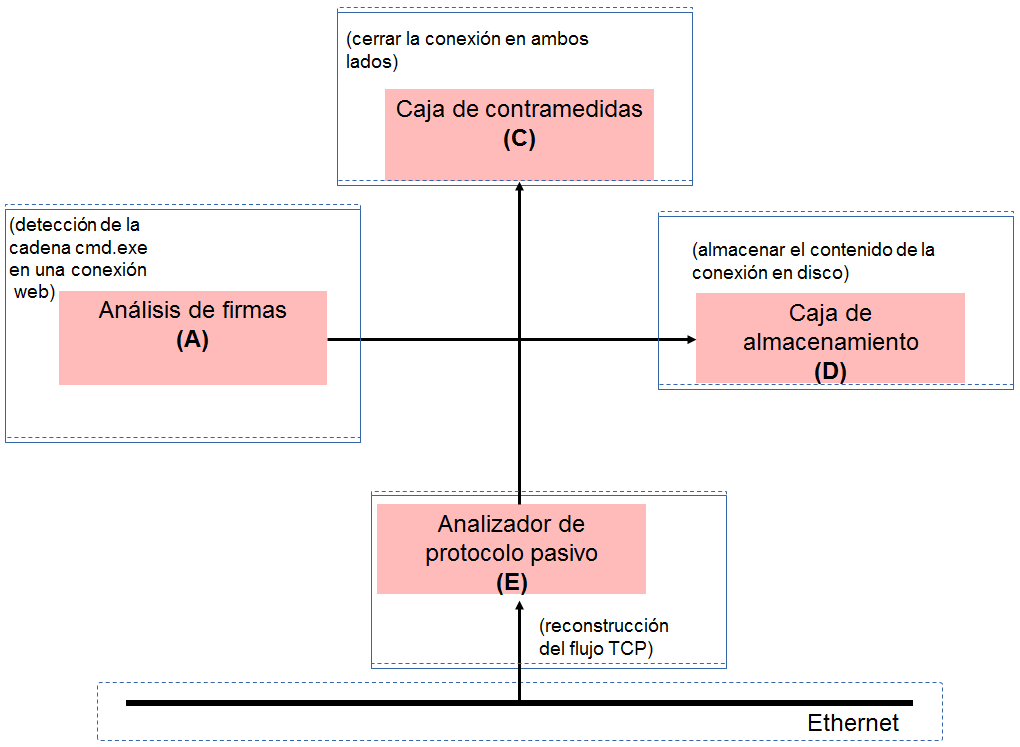
\includegraphics[scale=.4]{images/Arq_CIDF}
			\label{fig:IDS}
			\caption{Diagrama a bloques de la arquitectura CIDF.}
		\end{center}
	\end{figure}
	
	La arquitectura CIDF se debería tomar como referencia para tener como referencia los componentes que debería contener un IDS entre los diferentes fabricantes, sin embargo ésta no se ha considerado, ni como estándar, dentro del desarrollo de los IDSs debido a la complejidad de su lenguaje y el uso de GIDO para el intercambio de información.\\
	

	\subsubsection{Common Intrusion Specification Language}
	
	Describe un lenguaje que es puede ser usado para diseminar el registro de eventos, análisis de resultados y directivas de contra-medidas entre la detección de intrusos y los componentes de respuesta. Es la integración de los cuatro componentes de la arquitectura CIDF. Las capacidades básicas que esta arquitectura debe de cumplir son: \\
	
	\begin{itemize}
	
		\item \textbf{Información de eventos en bruto:} Consiste en una auditoría de registros y tráfico de red. Esta sección se encargaría de unir el módulo E con A.
		\item \textbf{Resultados de los análisis:} Son las descripciones de las actividades anómalas y de las intrusiones detectadas en el sistema. Une el equipo A con D.
		\item \textbf{Prescripciones de respuesta:} Acciones realizadas para detener un ciertas actividades anómalas modificando controles de seguridad. Une los módulos A y R.
		
	\end{itemize}
	
	El uso de la arquitectura CISL se ha considerado bastante complicado por la implementación de la arquitectura CIDF (que ya se había considerado compleja), por lo que no llegó a ser considerada por los fabricantes de IDSs.\\
	
	
	\subsubsection{Autopost de AusCERT}
	
	Tras la creación de las arquitecturas CIDF y CISL, el CERT de Austraila (AusCERT) desarrolló su propio sistema con el que se trabajarían los reportes, el cuál sería sencillo y que permitiría que se analizara y se generara un informe con el lenguaje Perl. La manera en que sería construido el reporte podría ser de la siguiente: \\ 
	
	\begin{lstlisting}
		Source: 216.36.45.84
		Ports: tcp 111
		Incident type: Network_scan
		re-distribute: yes
		timezone: GMT + 1300
		reply: no
		Time: Web 15 Mar 2000 at 14:01 (UTC) 
		
	\end{lstlisting}
	
	
	Debido a la facilidad de interpretación del Autopost, se tiene una gran interoperabilidad y es fácil de construir y de analizar. Este modelo al igual que los otros no fue tomado como un estándar debido a su escasa información reportada, ya que no era suficiente para los analistas de eventos, ya que estos requería de información detallada de los eventos para un análisis forense, por ejemplo.\\
	
	
	\subsubsection{Intrusion Detection Working Group}
	
	Debido a que el grupo de trabajo de ingeniería de internet (IETF\footnote{Organización internacional de normalización que tiene como objetivo hacer del Internet funcione mejor produciendo alta calidad, documentos técnicos relevantes que influencien la forma de diseñar, usar y manejar Internet para las personas \cite{IEFT}.} por sus siglas en inglés) rechazó las los enfoques de las arquitecturas CIDF y CISL, formó un equipo de trabajo llamado grupo de trabajo de detección de intrusos (IDWG por sus siglas en inglés) que como tal, no propusieron una arquitectura en específica, sino un modelo que se adaptara a las arquitecturas ya existentes. La proposición del IDWG fue: \\
	
	\begin{enumerate}[a)]
		\item El uso del lenguaje XML.
		\item Para una comunicación entre los módulos de la arquitectura, le uso de un servicio de mensajería IDMEF (Intrusion Detection Message Exchange Format).
		\item El uso de los protocolos IAP (Intrusion Alert Protocol) e IDXP (Intrusion Detection Exchange Protocol)
	\end{enumerate}
	
	Esta propuesta aún se encuentra en evaluación, la cuál contiene cuatro borradores para ser evaluados, explicando en qué consiste las etapas que la constituyen.\\
	
	\begin{itemize}
		\item IDWG			RFC 4766 (Requerimiento)
		\begin{list}{}{}
			\item El propósito de este es definir los formatos de información y procedimientos de intercambio para compartir información relevante entre IDSs, a de los sistemas de respuesta y a los administradores que estén en continua comunicación entre dichas partes y el IDS. Se requiere de un lenguaje que interpretar la semántica de otros IDSs en diferentes plataformas. La interacción entre el emisor y el receptor, debe tener implementadas formas de protección como un cifrado de los datos, debe pasar a través de un cortafuegos de manera transparente sin que se comprometa la seguridad del sistema de detección. Otras características deseables del comportamiento de los IDSs, es la automatización de las respuestas, donde las alertas sean compartidas entre los módulos del sistema empleando un formatos de prioridades para así, diferenciar los mensajes de intercambio generados habitualmente entre los módulos y las alertas de detección.\\
		\end{list}
		
		\item IDMEF-XML 	RFC 4765 (Intrusion Detection Message Exchange Format - XML)
		\begin{list}{}{}
			\item Este borrador describe el intercambio que se debe de llevar a cabo entre los IDSs a desarrollar utilizando el lenguaje \textit{XML}\footnote{Extensible Markup Language is un simple, muy flexible formato de texto derivado de del SGML (ISO 8879). Originalmente diseñado para conocer los retos de la edición electrónica a gran escala \cite{XML}.}. La implementación de este lenguaje para compartir datos relevantes entre los sistemas resulta más eficiente, debido a que la estructura que se usa para la lectura y escritura de dichos datos es mucho más fácil de hacerla. \\
		\end{list}
		
		\item BEEP TUNNEL	RFC 3620 (Block Extensible Exchange Protocol)
		\begin{list}{}{}
			\item Se plantea el uso de un proxy para la comunicación entre dos equipos de cómputo que se encuentren en diferentes redes. Por lo cual será empleado un túnel a través del proxy para que estos dos equipos en diferentes redes se puedan comunicar entre sí.\\
		\end{list}
		
		\item BEEP IDXP		RFC 4767 (Intrusion Detection Exchange Protocol)
		\begin{list}{}{}
			\item Se describen las normas que deben ser empleadas entre la comunicación de las entidades de los IDSs en diferentes redes. En donde el protocolo establece la creación de un sesión de un túnel BEEP para el cifrado de la comunicación y en donde la comunicación, punto a punto, sea de una manera transparente entre el paso de los proxies y así garantizar la confidencialidad de los datos transmitidos en el túnel. Los perfiles de alertas manejados por el IDXP operan dependiendo del nivel de la prioridad de la misma, pues cada nivel de prioridad de alertas tiene su propia sesión para la transmisión de éstas entre las entidades participantes (red, host, aplicación, etc.).\\
		\end{list}
		
	\end{itemize}
	
	
	Con base a lo mencionado anteriormente, se justifica el uso de este modelo. Pues la diferencia que tiene este con las arquitecturas antes descritas, se tiene que el objetivo del mismo es dar respuesta a la interoperabilidad que se debe de llevar a cabo entre los diferentes fabricantes de IDSs. Con ello, sugiriendo que la comunicación entre los componentes, y la generación de los reportes, puedan ser adaptados a las necesidades de los datos de interés requeridos del sistema que se protege. Para poder llevar a cabo los puntos mencionados, se puede hacer gracias a las características que ofrece el lenguaje XML, ya que fue diseñado como un estándar para el intercambio de información multiplataforma, ofreciendo una compatibilidad entre sistemas.